%!TEX root = ../PhDThesis.tex



% *********************************************************************************************************************
\chapter{Fragments from the second study}\label{app:fragments-cafe}
% *********************************************************************************************************************



\resubmission{This appendix is new, and includes the complete fragments from the cafe talk chapter}
This appendix includes the full fragments presented over a number of excerpts in \autoref{ch:empirical cafe}. There are three fragments:

\begin{itemize}
    \item \appref{app:fragments-cafe sunset} is the transcript for the \textit{When Does the Sun Go Down?} fragment, which is composed of Data Excerpts \ref{frag:empirical cafe findings newinfo-i}, \ref{frag:empirical cafe findings newinfo-ii}, and \ref{frag:empirical cafe findings newinfo-iii};
    \item \appref{app:fragments-cafe animals} is the transcript for the \textit{Do Animals Have Accents?} fragment, which is composed of Data Excerpts \ref{frag:empirical cafe findings answering-i}, \ref{frag:empirical cafe findings answering-ii}, \ref{frag:empirical cafe findings answering-iii}, and \ref{frag:empirical cafe findings answering-iv}; and
    \item \appref{app:fragments-cafe mama} is the transcript for the \textit{Hey Siri! \ldots Call My Mother} fragment, which is composed of Data Excerpts \ref{frag:empirical cafe findings capability-i} and \ref{frag:empirical cafe findings capability-ii}.
\end{itemize}

% *********************************************************************************************************************

\section{When Does the Sun Go Down?}\label{app:fragments-cafe sunset}
\begin{inlinefrag} 
    \begin{transcript}
        \by HAR {i’ll be fine in like three minutes ((holds hands in front of} \\
        \by     {eyes))} \\
        \by RES {keeps coming back as well like} \\
        \by SAL {as soon as you cha\emph{nge} it comes back} \\
        \by JUL {yeah yeaha} \\
        \later  {0.3} \\
        \by RES {there’s actually just someone out there with a light!} \\
        \by ALL {((laugh))} \\
        \later {\ldots}[7] \\
        \by JUL {[ ((removes cover from device but leaves open)) ]} \\
        \by SAL {((laughs))} \\
        \by JUL {((presses button on device))} \\
        \by HAR {there we go!} \\
        \by JUL {\textbf{what’s the time of sunset?}} \\
        \later  {1.3} \\
        \by ALL {((gaze at the tablet))} \\
        \later  {3.0} \\
        \by JUL {ok! \textit{// ((device displays clock)) //}} \\
        \by ART {((leans in to look))} \\
        \by SAL {that’s [ a~~~~~~] fucking analogue clock it pisses me off!} \\
        \by HAR {~~~~~~~[ today? ]} \\
        \by HAR {ilunno (0.6) 24 hour=} \\
        \by JUL {<no no no!> it misunderstood actually (0.8) understood what’s} \\
        \by     {the [ time ]} \\
        \by HAR {~[ time ] now} \\
        \by JUL {so-} \\
        \by ART {soaoah yeah\intUp} \\
        \by JUL {shall i ask (1.6) um:=} \\
        \by HAR {~~~~~~~~~~~~~~~~~~~~~=what time will the [ sun set? ]} \\
        \by JUL {~~~~~~~~~~~~~~~~~~~~~~~~~~~~~~~~~~~~~~~~~[ ((holds button)) ]} \\
        \by JUL {\textit{// ((audible chime)) //}} \\
        \later  {4.0} \\
        \by JUL {\textit{ // ((on screen text: go ahead i’m listening\ldots)) //}} \\
        \later  {0.3} \\
        \by JUL {\textbf{when does the sun go down?}} \\
        \later  {2.9} \\
        \by JUL {sunset will be at [ seventeen thirty two ]} \\
        \by ART {~~~~~~~~~~~~~~~~~~[ ther:::e you go~~~~~~]} \\
    \end{transcript}
    \begin{center}
            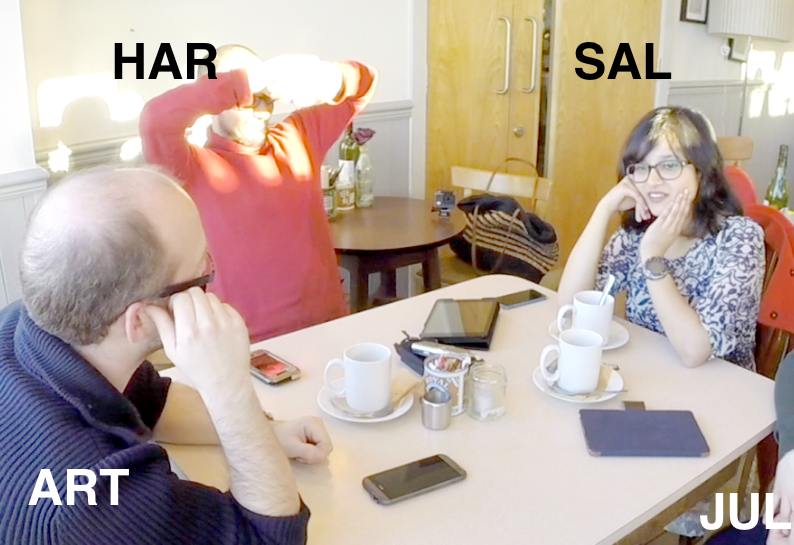
\includegraphics[width=.5\linewidth]{Graphics/3-2-Empirical-Cafe/FragmentSunset-1}\\
            (line 1)\\[1cm]
            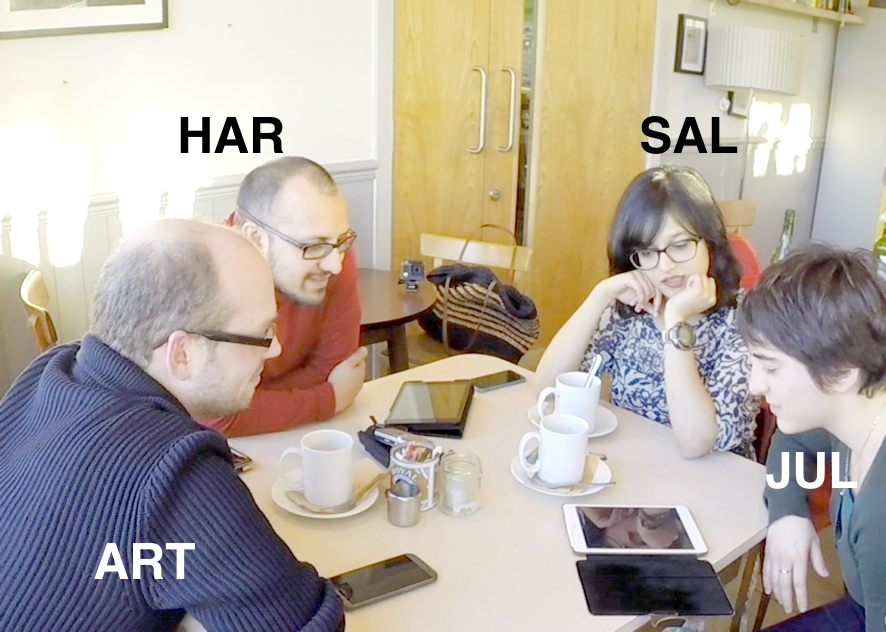
\includegraphics[width=.5\linewidth]{Graphics/3-2-Empirical-Cafe/FragmentSunset-2}\\
            (line 25)
    \end{center}
\end{inlinefrag}

% *********************************************************************************************************************



\section{Do Animals Have Accents?}\label{app:fragments-cafe animals}
\begin{inlinefrag} 
    \begin{transcript}
        \by KAR {do cats acth- (0.5) can you work out whether it's french because} \\
        \by     {because its talking in a- doing a french cat impression} \\
        %\im    1 {Graphics/3-2-Empirical-Cafe/FragmentAnimals-1.png}
        \by LIL {i::::: think some animals you can} \\
        \later {1.9} \\
        \by LIL {((picks up phone from table))} \\
        \later {\ldots}[34] \\
        \by LIL {er:::m: ((holding phone in front of her at chest level))} \\
        \later  {3.7} \\
        %\im    3 {Graphics/3-2-Empirical-Cafe/FragmentAnimals-2.png}
        \by LIL {((moves phone up to face)) \textbf{do animals have acce\emph{nts}?}} \\
        \later  {2.1} \\
        \by GAR {((shifts gaze to LIL))} \\
        \by     {yes they do actually! i think i've read something} \\
        \by LIL {i think i have [ too\intDown{}~~]} \\
        \by GAR {~~~~~~~~~~~~~~~[ yeas!~] [ (0.6) \emph{cows}! i- i~~~~~~~~~~~~~~~]} \\
        \by     {~~~~~~~~~~~~~~~~~~~~~~~~~read about cows that they have} \\
        \by     {~~~~~~~~~~~~~~~~~~~~~~~~~different accents around the world} \\
        \by KAR {~~~~~~~~~~~~~~~~~~~~~~~~~[ you missed mine- my racist joke ]} \\
        \by LIL {\textbf{DO: \emph{ANIM}ALS HA\emph{V}E \emph{ACCEN}TS!}} \\
        \later  {2.4} \\
        \by LIL {°rubbish°=} \\
        \by KAR {~~~~~~~~~~~=parrots presumably do=} \\
        \by LIL {~~~~~~~~~~~~~~~~~~~~~~~~~~~~~~~~~~=can you ask it?} \\
        \by     {((holds phone out in front of KAR's face))} \\
        %\im    1 {Graphics/3-2-Empirical-Cafe/FragmentAnimals-3.png}
        \by RES {((retrieves phone out of pocket))} \\
        \by KAR {\textbf{DO: ANI\emph{MALS} HAVE ACC::\emph{ENT}S!}} \\
        \later  {0.9} \\
        \by LIL {no:!} \\
        \by RES {\textit{//~sorry i'm-~//}} \\
        \by RES {((RES touches screen to stop utterance))} \\
        \by RES {\textbf{do animals have accents?}} \\
        \by LIL {\textbf{d\emph{o:} \emph{anim}als ha\emph{v}e a\emph{ccents}?}} \\
        \by RES {\textit{//~ok i've found this on the web~//} (sigh)} \\
        \by GAR {do [ they?~~]} \\
        \by LIL {~~~[ ah (.) ] it's working now!} \\
    \end{transcript}

    \begin{center}
            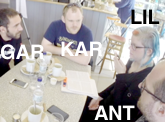
\includegraphics[width=.7\linewidth]{Graphics/3-2-Empirical-Cafe/FragmentAnimals-2}\\
            (line 44)\\[1cm]
            
\includegraphics[width=.7\linewidth]{Graphics/3-2-Empirical-Cafe/FragmentAnimals-3}\\
            (line 56)
    \end{center}
\end{inlinefrag}

% *********************************************************************************************************************

% *********************************************************************************************************************



\section{Hey Siri! \ldots Call My Mother}\label{app:fragments-cafe mama}
\begin{inlinefrag*} 
    \begin{transcript*}
        \by GAR {i'm curious if I say in} \\
        \by     {romanian (.) to call my mother} \\
        \later {0.7} \\
        \by GAR {it will actually find the } \\
        \by     {contact for my mother is (.)} \\
        \by     {mama in romanian (.) if I say} \\
        \by     {call my mum will it actually} \\
        \by     {call my mother which is in a} \\
        \by     {contact as mama (0.7) will it} \\
        \by     {make the connection between} \\
        \by     {mama and mum} \\
        \by RES {cos you can also tell people} \\
        \by     {who they (.) like you can say} \\
        \by     {like\vspace*{1cm}} \\
        \im 1   {Graphics/3-2-Empirical-Cafe/FragmentMamma-1.png}
        \by GAR {\textbf{hey siri=}} \\
        \by RES {~~~~~~~~~=my mother is this} \\
        \by     {~~~~~~~~~~person (0.8)} \\
        \by GAR {((glances down at screen))} \\
        \by     {((moves device in front of} \\
        \by     {mouth)) \textbf{hey siri}} \\
        \by GAR {((moves device to chest} \\
        \by     {height between the two))} \\
        \later  {1.0} \\
        \by RES {i'd press the button} \\
        \later  {1.2} \\
        \by GAR {((moves device in front of} \\
        \by     {mouth)) \textbf{hey siri}} \\
        \by GAR {((moves device to chest} \\
        \by     {height between the two))} \\
        \later  {2.4} \\
        \by GAR {((moves device in front of} \\
        \by     {mouth)) \textbf{call my \emph{m}other}} \\
        \im 1   {Graphics/3-2-Empirical-Cafe/FragmentMamma-2.png}
        \by     {((GAR and RES look at screen))}  \\
        \later  {5.9} \\
        \by     {\textit{// what is your mother's}} \\
        \by     {\textit{~~~name? //}} \\
        \by RES {((points towards screen)) yeah} \\
        \by     {but then} \\
        \later  {0.9} \\
        \by GAR {\textbf{my mother is mama}} \\
        \by GAR {\textit{// i can’t find anyone called}} \\
        \by     {\textit{~~~mamma //}} \\
    \end{transcript*}
\end{inlinefrag*}

% *********************************************************************************************************************
